\documentclass[12pt]{article}
\usepackage[utf8]{inputenc}
\usepackage[top=0.75in, bottom=0.75in, left=0.75in, right=0.75in, headheight=15pt]{geometry}
\usepackage{amsmath, amssymb, amsthm, graphicx, hyperref, enumerate, multirow,  multicol, tikz, centernot, cancel, forest, lipsum, mathtools, bm, esvect, fancyhdr, esdiff, float, parskip, comment}

\DeclareMathSymbol{*}{\mathbin}{symbols}{"01} % change * to /cdot inside math
% \begingroup % let only this align, etc. break across pages
% \allowdisplaybreaks
% \begin{align}
%     ....
% \end{align}
% \endgroup

% \begin{figure}[H]
%     \centering
%     \includegraphics{}
%     \caption{}
%     \label{fig:}
% \end{figure}

% \texorpdfstring{$k$}{k} math inside (sub/)section label

\pagestyle{fancy}
\fancyhead[L]{Liheng Cao}
% \fancyhead[C]{center}
\fancyhead[R]{}

\title{} % title
\author{Liheng Cao} % name
\date{\today} % custom date else today's date

\begin{document}
\maketitle

\section{}
\begin{enumerate}[(a)]
	\item \begin{figure}[H]
		\centering
		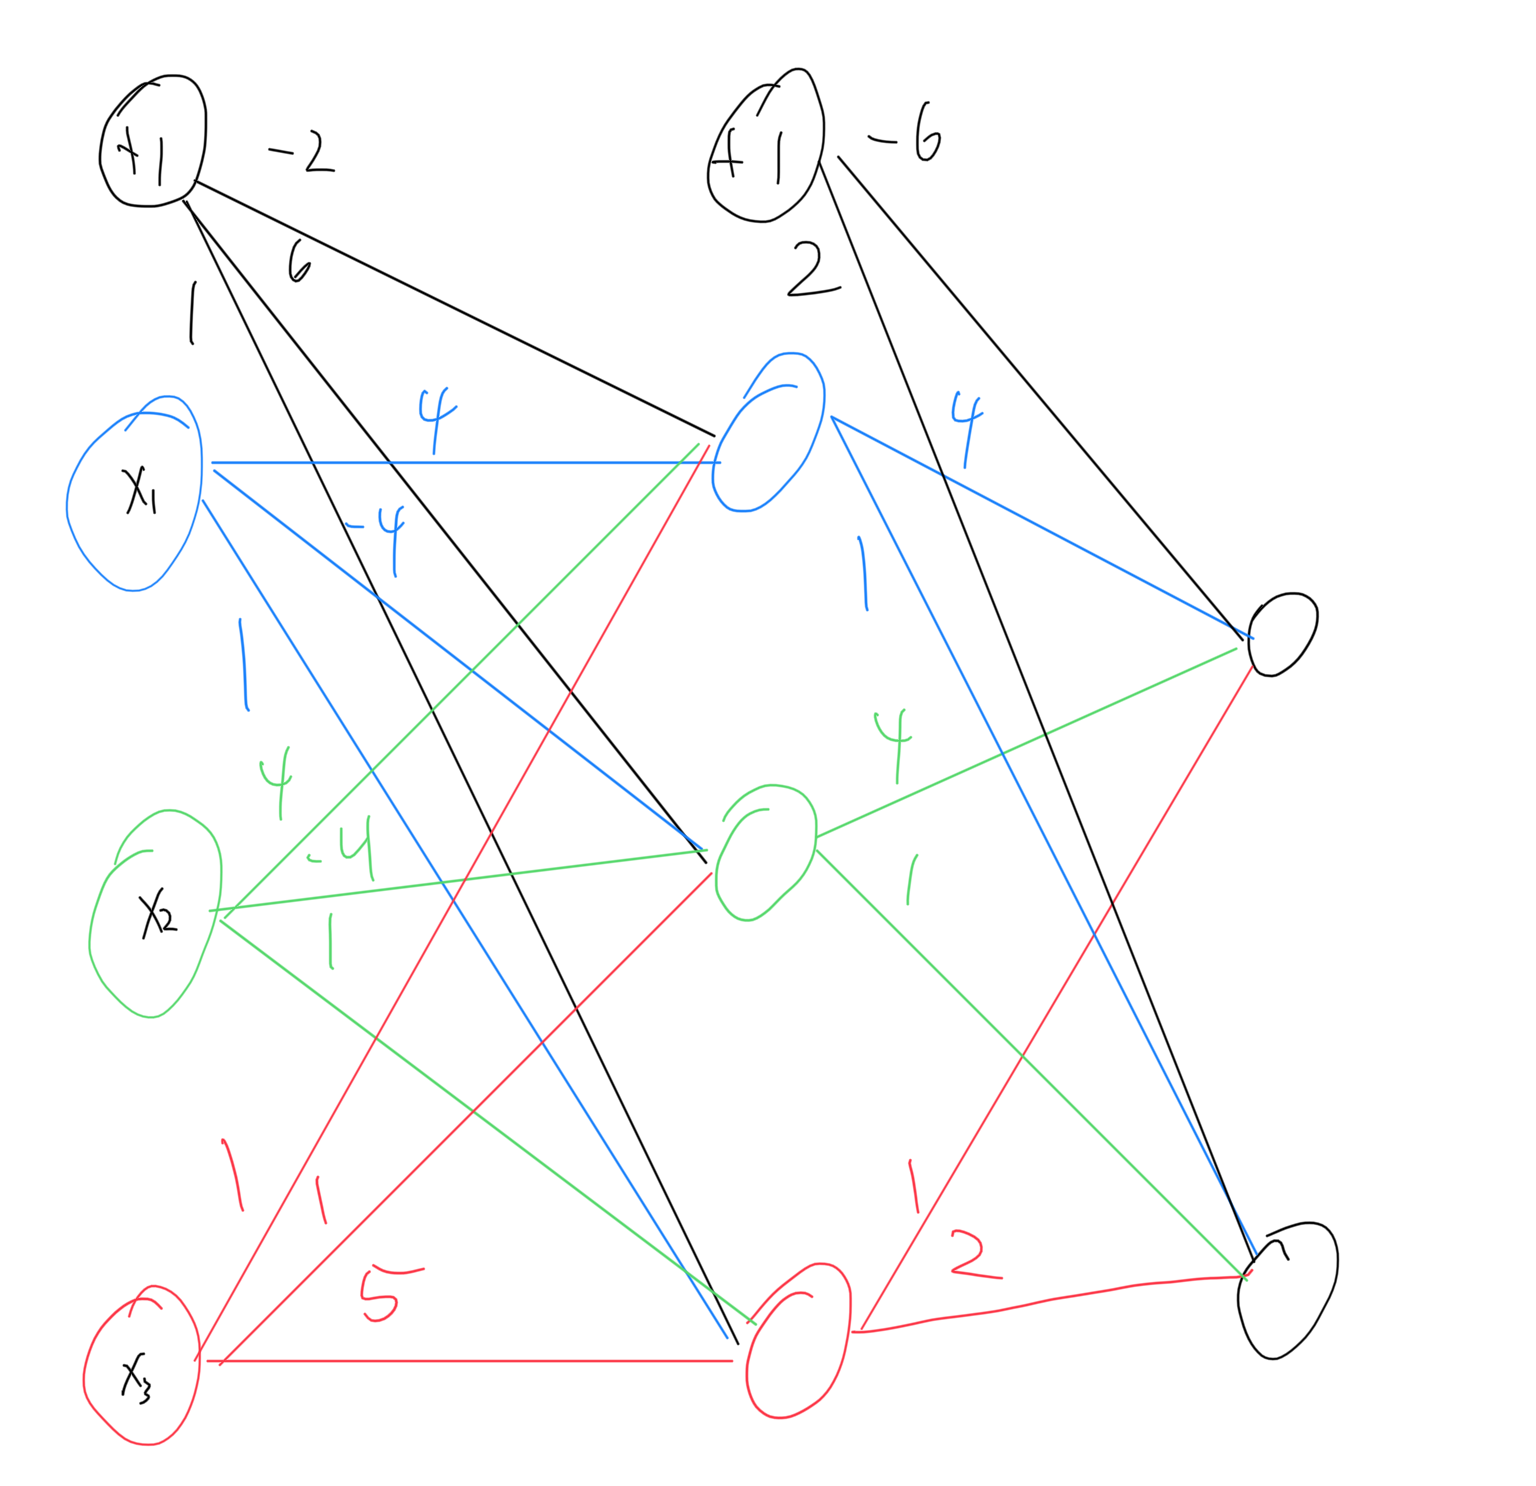
\includegraphics[width=\textwidth*2/3]{images/1a.png}
		\caption{Drawing of Neural Network}
		\label{fig:1:a}
	\end{figure}
	
	\item 
\end{enumerate}

\end{document}